\documentclass[tikz,border=8pt]{standalone}
\usepackage[scaled=0.95]{helvet}
\renewcommand{\familydefault}{\sfdefault}
\usepackage[europeanresistors,americanvoltages]{circuitikz}
\definecolor{TEJNavy}{HTML}{1E2B55}
\definecolor{TEJBlue}{HTML}{1769AA}
\begin{document}
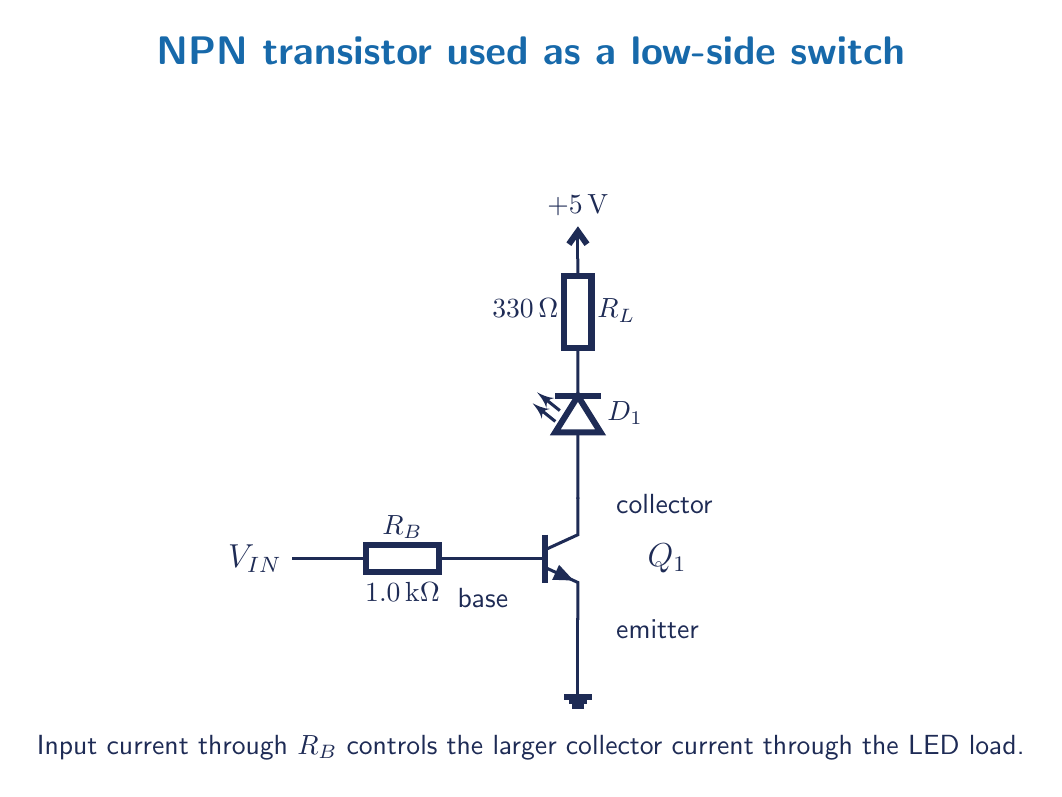
\begin{tikzpicture}[line width=1.1pt,draw=TEJNavy,text=TEJNavy,font=\sffamily]
  \ctikzset{bipoles/length=1.15cm}

  \node[font=\bfseries\Large,text=TEJBlue] at (3.7,8.0)
    {NPN transistor used as a low-side switch};
  \node[npn,scale=1.2] (Q1) at (4.3,1.55) {};
  \node[anchor=west,font=\large] at (5.05,1.55) {$Q_1$};
  \draw (Q1.E) -- ++(0,-0.65) node[ground] {};
  \draw
    (Q1.C) -- ++(0,0.45)
    to[leD,l_={$D_1$}] ++(0,1.25)
    to[R,l_={$R_L$},a^={$330\,\Omega$}] ++(0,1.35)
    node[vcc] {$+5\,\mathrm{V}$};
  \draw
    (Q1.B) to[R,l_={$R_B$},a^={$1.0\,\mathrm{k}\Omega$}]
    ++(-2.8,0) node[left,font=\large] {$V_{IN}$};
  \node[anchor=west] at (4.65,2.25) {collector};
  \node[anchor=west] at (4.65,0.65) {emitter};
  \node[anchor=east] at (3.55,1.05) {base};
  \node[align=center] at (3.7,-0.85)
    {Input current through $R_B$ controls the larger collector current through the LED load.};
\end{tikzpicture}
\end{document}
